

\chapter{Seleção de Correias Trapezoidais}


A seleção de correias se inicia com a definição dos parâmetros fundamentais do sistema de transmissão, sendo eles:

\begin{itemize}
    \item Potência a transmitir
    \item Rotação dos eixos
    \item Características do acionamento
    \item Estimativa de distância entre eixos
\end{itemize}

Pode-se dividir o processo de escolha em alguns passos bem definidos:

\section{Passo 01 - Definição da potência de projeto}

Com base na potência nominal, pode-se estimar a potência efetiva, com base nas condições de serviço, representadas por ${K_0}$.

\begin{equation}
    P_P=K_0\cdot N_0 \label{9.24}
\end{equation}

Os valores para ${K_0}$ são obtidos a partir da seguinte tabela:

\begin{figure}[h]
	\centering
	\caption{Fator de Serviço}
    \label{k0_tabela}
	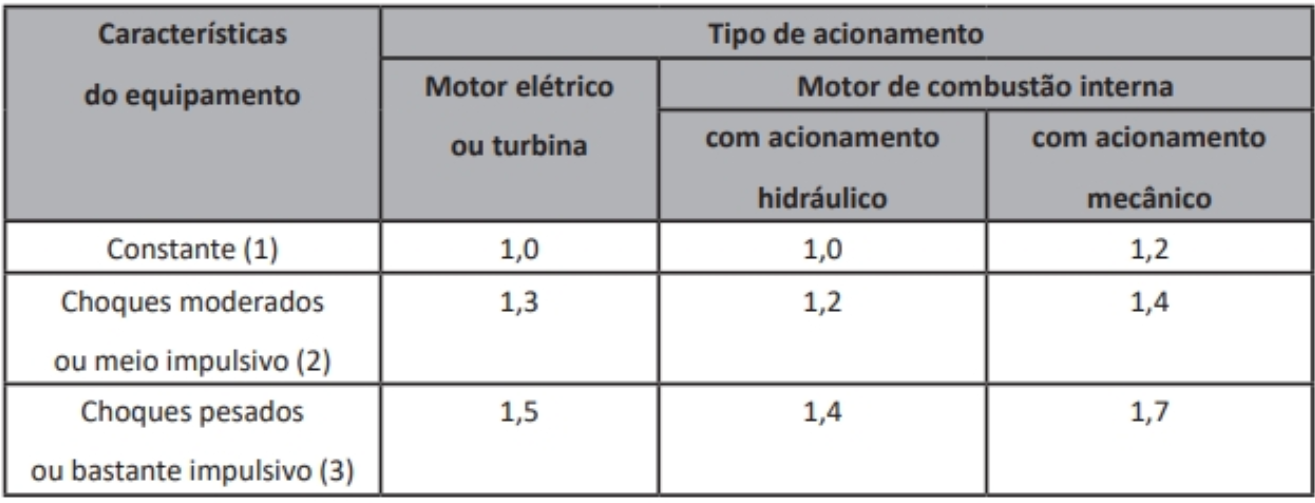
\includegraphics[scale=0.4]{Imagens/K0.png}
	\fonte{\cite{EMA_Barbieri}}
\end{figure}

\newpage
\section{Passo 02 - Definição do perfil da Correia}

Com base na potência e na rotação do eixo, pode-se utilizar a Figura~\ref{graf_perfis} para definir o perfil da correia

\begin{figure}[h]
	\centering
	\caption{Gráfico de seleção para correias trapezoidais.}
    \label{graf_perfis}
	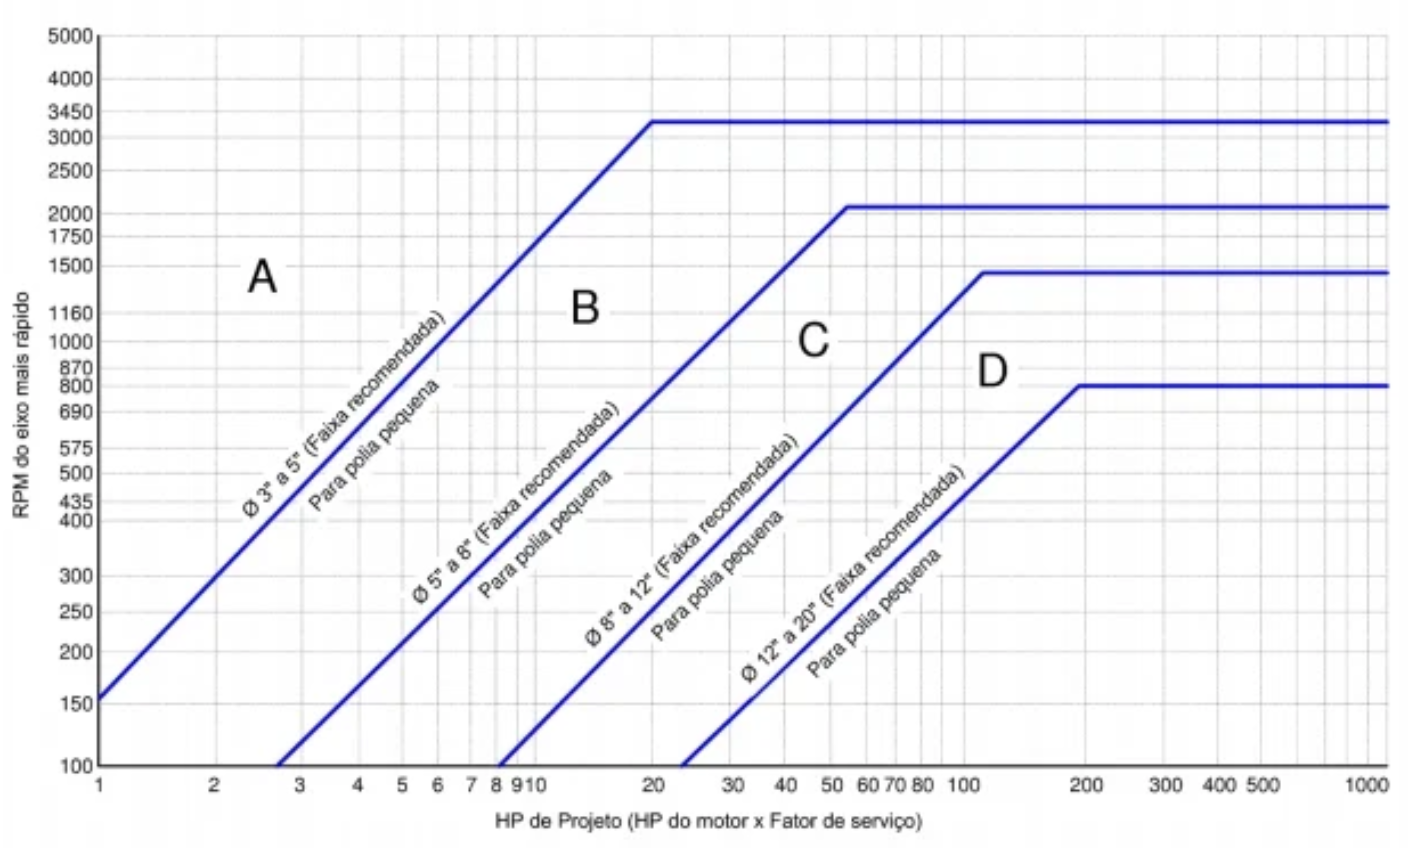
\includegraphics[scale=0.42]{Imagens/graf_perfis.png}
	\fonte{\cite{EMA_Barbieri}}
\end{figure}

\begin{figure}[h]
	\centering
	\caption{Opções de perfis de Correia}
    \label{perfis_correia}
	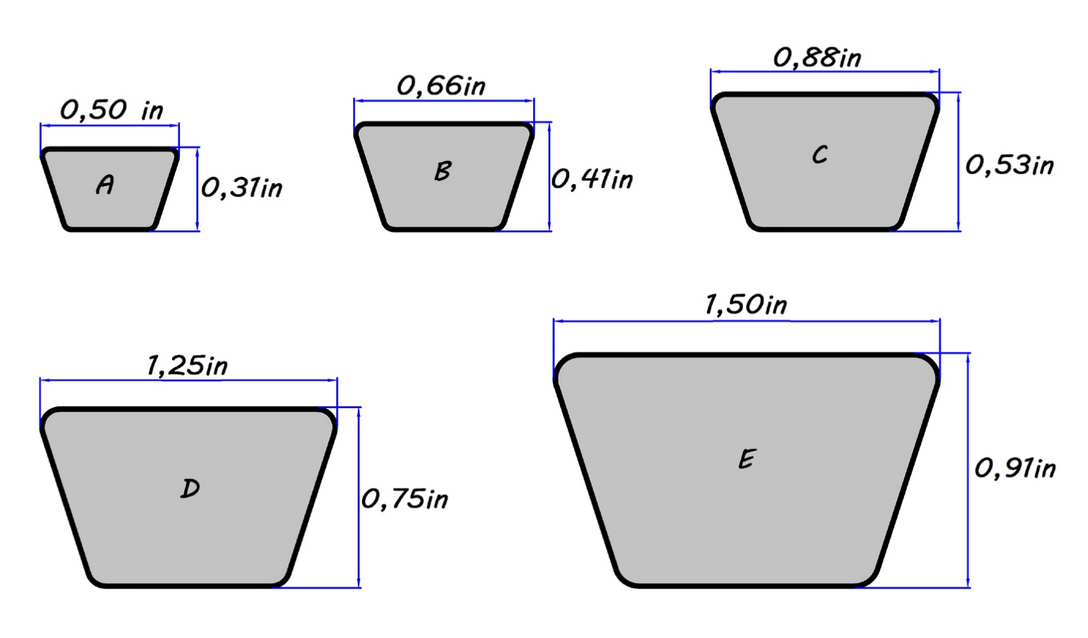
\includegraphics[scale=0.45]{Imagens/perfis_correia.png}
	\fonte{\cite{EMA_Barbieri}}
\end{figure}

\section{Passo 03 - Definição dos diâmetros das Polias}

Caso não haja definição do diâmetro da polia motora, deve-se adotar o diâmetro recomendado pela Figura~\ref{graf_perfis}. A polia movida é determinada a partir da razão de transmissão necessária.

\section{Passo 04 - Definição da velocidade tangencial da correia}

Possuindo todos os dados do sistema, pode-se calcular a velocidade da correia utilizando a Eq.~\eqref{v_correia}.

\begin{equation}
    v=w \cdot r_p=\frac{\pi \cdot d_p \cdot n}{60} \label{v_correia}
\end{equation}

Em termos práticos, a velocidade a correia não deve ultrapassar 20 m/s.

\section{Passo 05 - Definição do comprimento da correia e do ângulo de abraçamento da polia}

Com a definição dos diâmetros das polias e a distância entre centros pode-se calcular o comprimento da polia:

Abertas:
\begin{equation}
    L=2a + 1,57(dp_2+dp_1)+ \frac{(dp_2-dp_1)^{2}}{4a} \label{comprimento_correia}
\end{equation}

\bigskip
Cruzadas:
\begin{equation}
    L=2a + 1,57(dp_2+dp_1)+ \frac{(dp_2+dp_1)^{2}}{4a}
\end{equation}

\bigskip
E também o ângulo de contato:

\begin{equation}
    \theta=\pi \pm 2arcsen \left( \frac{dp_2 - dp_1}{2a} \right)
\end{equation}



\section{Passo 06 - Definição do comprimento padronizado da correia e correção da distância entre centros}

O comprimento da correia deve ser aproximado em um comprimento comercial, encontrado na Tabela~9.13 de \cite{EMA_Barbieri}. A diferença entre o comprimento original e o padronizado será corrigida na distância entre centros com base na Eq. \eqref{deixo}.

\begin{equation}
    a_{conv}=a-\left(\frac{L-L_{tab}}{2}\right)     \label{deixo}
\end{equation}


\section{Passo 07 - Determinação dos fatores de correção}

A fim de acomodar propriamente as correias padronizadas, pequenos ajustes nos ângulos de contato e comprimento devem ser realizados, utilizando as Figuras~\ref{correcao_arco} e \ref{correcao_comprimento}


\begin{figure}[h]
	\centering
	\caption{Fator de Correção Arco}
    \label{correcao_arco}
	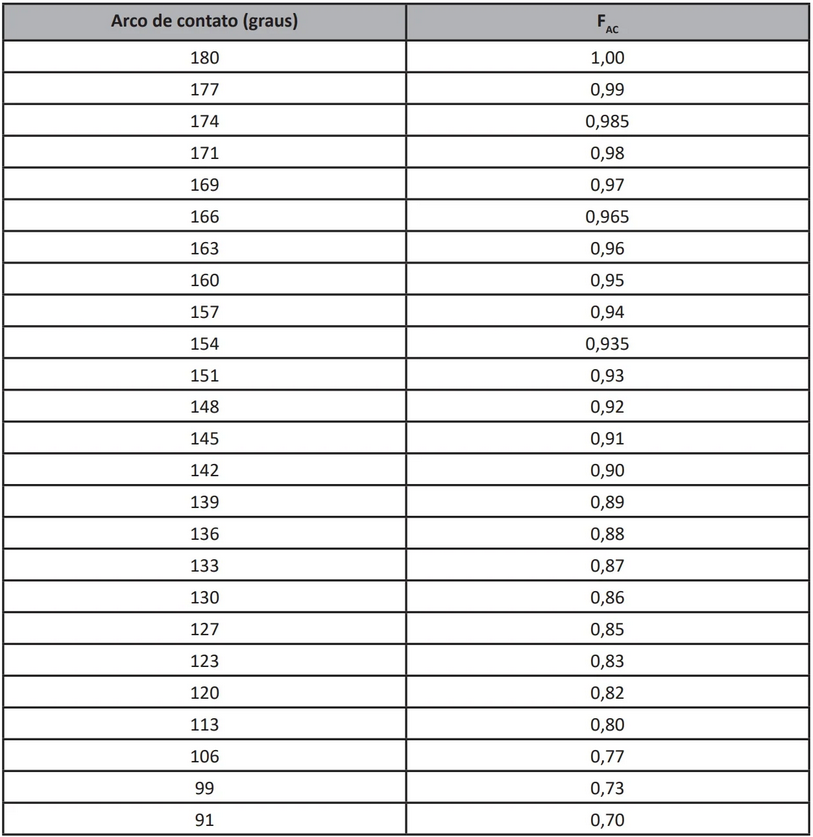
\includegraphics[scale=0.7]{Imagens/correcao_arco.png}
	\fonte{\cite{EMA_Barbieri}}
\end{figure}


\begin{figure}[p]
	\centering
	\caption{Fator de Correção Comprimento}
    \label{correcao_comprimento}
	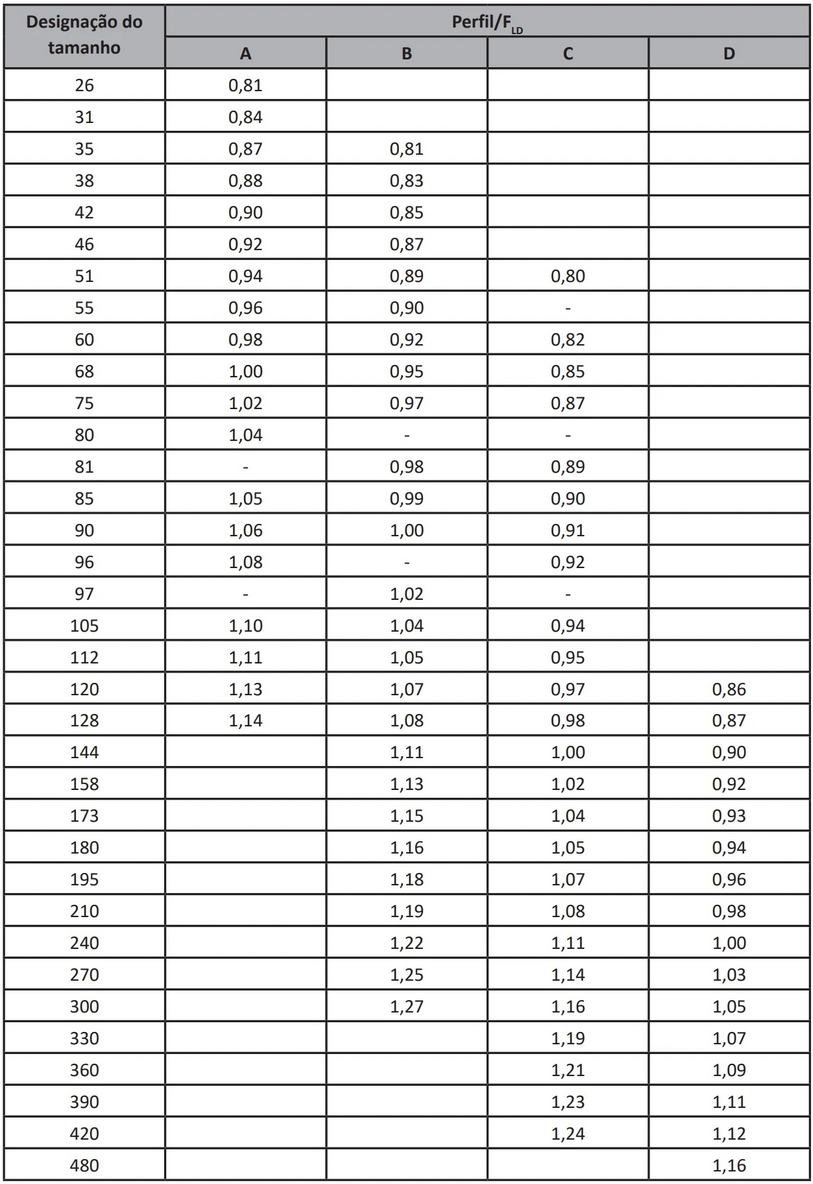
\includegraphics[scale=0.7]{Imagens/correcao_comprimento.png}
	\fonte{\cite{EMA_Barbieri}}
\end{figure}

\pagebreak
\section{Passo 08 - Determinação do HP básico e do HP adicional por correia}

Dada designação de correia possui parâmetros máximos de operação, utilizando as tabelas 9.6 a 9.9 e 9.6A a 9.9A de \cite{EMA_Barbieri}, pode-se estimar a potência básica e adicional

\begin{equation}
    HP_{class} = HP_{bas} + HP_{adic}
\end{equation}

\section{Passo 09 - Determinação do HP efetivo e do número de correias}

Com os fatores de correção em mãos, juntamente com os valores de potência, pode-se estimar a potência efetiva.
Também seno possível definir o número de correias necessárias para o projeto.


\begin{align}
    HP_{\text{efet}} &= HP_{\text{class}} \cdot F_{AC} \cdot F_{LP} \\
    N_{\text{correias}} &= \frac{P_p}{HP_{\text{efet}}}
\end{align}
